%% The basic ESPResSo tutorial
%%
% Writer's guide lines:
% - provide background information and references
% - do not get lost in details but maintain a nice readability
% - describe every line of the script, that contains an ESPResSo
%   command (in future tutorial, only describe new ones)
%
%%%%%%%%%%%%%%%%%%%%%%%%%%%%%%%%%%%%%%%%%%%%%%%%%%%%%%%%%%%%%%%%%
%%%%%%%%%%%%%%%%%%%%%%%%%%%%%%%%%%%%%%%%%%%%%%%%%%%%%%%%%%%%%%%%%
% From the brainstorming:
%
% Preknowledge:
%
% Basic MD(simple integrator,langevin thermostat, ---basic tcl
% basic potentials, basis tutorial 1
%
% Basis Tutorial: written in Latex
%
% <<every line of script code should be explained>>
%
% 1) tcl basic setting up a system
% MD, soft sphere and Lennard-Jones Fluid (argon system),
% Units
%
% online visualization (pdb output)
% rdf, pressure,energy,
%
% online analysis function
% savin, readin writeout, offline analysis, statistics
%
% Structure:
% Part1:
% 1) Prerequisits (what you should know beforehand: basic tcl knowledge,
% Here you can find more info: Allen, Tildesley: Frenkel smit,
% Rappaport, tcl tutorial,
%
% 2) Physics of the systems (argon, soft sphere system)
%
% 3) Algorithms (verlocity verlet, Langevin, Potentials, LJ)
% 3b) about units
%
% Part2
% 1) simulation script in all detail, line by line
% Initialize
% Visualize
% Simulate (with online analysis, saves for later off-line analysis,
% (Savelize (save our lives ))
%
% 2) a new script for later
% analysis, and other helper ideas
%
% Things to remember and take care of:
% Use the same names for variables
%
% ====================================================================
% General Tutorial: (the next tutorials: pe_solution, cell model of one
% charged colloid, LB, ferrofluid)
%

% basiert auf KOMA-Script scrbook-Klasse
\documentclass[11pt,a4paper,% BCOR8mm,
	       %twoside, onecolumn, openright, cleardoubleempty, %
	       %parindent,
headnosepline, footnosepline, notitlepage, %
	       %onelinecaption,
bigheadings, % bibtotoc, %tocindent, listsindent, %
	       %chapterprefix, noappendixprefix,
	       %tablecaptionbelow,
	       %pointlessnumbers, % macht Probleme (Anhang ohne Punkt, aber sonst Kapitel mit Punkt
	       % abstractoff, fleqn, leqno,
	       % openbib, origlongtable,
final]{scrartcl}

% Satzspiegel

% wenn keine KOMA-Klasse verwendet wird, kann so der Satzspiegel
% berechnet werden
%\usepackage[DIV15,BCOR12mm,pagesize]{typearea}

% Hier knnen Seitenhoehe und -breite individuell angepasst werden
%\areaset[BCOR]{Breite}{Hohe}
% oder
%\usepackage[a4paper,body={15.6cm,23cm},left=3cm]{geometry}

% ============================================================================

%% Grafikpakete
% Fr einfache Einbingung von Grafiken
\usepackage{graphicx}%
\usepackage{framed, color}

% Wenn man direkt mit dem pdflatex eine PDF-Datei erzeugt, sollten diese beiden
% Pakete eingebunden werden (Hyperlinks, bessere Bildschirmschriftarten usw.)
\usepackage{color}
\definecolor{mylinkcolor}{rgb}{0.5812,0.0665,0.0659} % IndianRed
\definecolor{mycitecolor}{rgb}{0.075,0.31,0.0431} % MossGreen
\definecolor{myurlcolor}{rgb}{0.0118,0.098,0.7412} % DarkBlue
\usepackage[pdftex,bookmarks]{hyperref}

% Druckversion
% f�r reine pdf-Dateien noch Option colorlinks hinzufgen, um Links farbig zumachen
% \usepackage[pdftex,bookmarks,bookmarksopen,citecolor={mycitecolor},%
%  linkcolor={mylinkcolor},urlcolor={myurlcolor},breaklinks=true,%
%  hypertexnames=false,hyperindex=true,encap,colorlinks]{hyperref} %

%  	\hypersetup{
%     pdftitle = {},
%     pdfauthor = {Kai Grass},
%     pdfsubject = {},
%     pdfkeywords = {},
%     pdfcreator = {},%
%     pdfproducer = {},
% 	}%

\usepackage{ae,aecompl}

% ============================================================================

%% Sprachliche Pakete
\usepackage[english]{babel}
% Neue Deutsche Rechtschreibung
%\usepackage[ngerman]{babel}
%\usepackage{ngerman}

% Paket zur einfacheren Eingabe deutscher Umlaute
%\usepackage[applemac]{inputenc} %Mac
\usepackage[latin1]{inputenc}   %UNIX/LINUX
% \usepackage[ansinew]{inputenc}  % Windows
\usepackage[T1]{fontenc}

% ============================================================================

% Literaturverzeichnis
\usepackage[square,numbers,sort&compress]{natbib}
%\usepackage{bibmods}
%\bibpunct{(}{)}{,}{a}{}{,}
%\bibpunct{(}{)}{,}{a}{,}{;}
\setlength{\bibsep}{1ex}

% ============================================================================

% Stichwortverzeichnis
% \usepackage{makeidx}
% \makeindex

% ============================================================================

% Deutsche Zahlenkonvention (1 (Komma) 0 statt 1 (Punkt) 0)
% \usepackage{ziffer}

%% Schriftarten
\usepackage{times} % times is used to avoid bitmap fonts in PDF

%% Mathematische Packages
% Dieses Pakete definiert viele ntzliche mathematische Befehele und
% Die Option "intlimits" bewirkt, dass beim Integral die Grenzenangaben oben
% und unten erscheinen und nicht seitlich.
\usepackage[intlimits]{amsmath}
\usepackage{amsfonts}
\usepackage{amsthm}
\usepackage{mathrsfs}
\usepackage{stmaryrd}


% Diese Schriftarten ermglichen schne Mengensymbole fr natrliche Zahlen, usw.
% siehe Definition von \N, \Z usw. Dies ist Geschmackssache.
%\usepackage{bbm}
%\usepackage{dsfont}

% Subfigures
\usepackage{subfigure}

% Needed for Tabular-Umgebung
\usepackage{array}

% werden (sog. Schusterjungen und Hurenkinder vermeiden)
%\clubpenalty = 10000
%\widowpenalty = 10000

\sloppy

% Ein Paket um "kommutative Diagramme" zu erstellen. Fuer einfhrende Beispiele
% siehe xymanual.ps und xyreference.ps
%\usepackage[all]{xy}

%%%%%%%%%%%%%%%%%%% Shortcuts %%%%%%%%%%%%%%%%%%%%%%%%%%%%%%%%%%%%%%%%%%%%
%\newcommand{\N}{\mathbbm{N}}	% Natuerliche Zahlen
%\newcommand{\Z}{\mathbbm{Z}}	% Ganze Zahlen
%\newcommand{\Q}{\mathbbm{Q}}	% Rationale Zahlen
%\newcommand{\R}{\mathbbm{R}}	% Reelle Zahlen
%\newcommand{\C}{\mathbbm{C}}	% Komplexe Zahlen
%\newcommand{\one}{\mathbbm{1}}	% Einheits Eins
%
%\newcommand{\toinf}{\to\infty}				% --> oo
%\newcommand{\tozero}{\to 0}				% --> 0
%\newcommand{\ontop}[2]{\genfrac{}{}{0pt}{}{#1}{#2}}	% Aufeinander
%\newcommand{\abs}[1]{\left|#1\right|}
%\newcommand{\argmax}{\mathop{\rm arg\,max}}

% Ein Befehl, um Abbildungen einfach einheitlich zu gestalten
% Bsp: \abb{f}{\R}{\R}{x}{x^2}

%\newcommand{\abb}[5]{%
%\setlength{\arraycolsep}{0.4ex}%
%\begin{array}{rcccc}%
%#1 &:\,& #2 & \,\,\longrightarrow\,\, & #3 \\[0.5ex]%
%     & & #4 & \longmapsto & #5%
%\end{array}%
%}

%%%%%%%%%%%%%%%%%%% Theorem definitions %%%%%%%%%%%%%%%%%%%%%%%%%%%%%%%%%%
%\theoremstyle{plain}
%\newtheorem{theorem}{Theorem}[chapter]
%\newtheorem{proposition}[theorem]{Proposition}
%\newtheorem{lemma}[theorem]{Lemma}
%\newtheorem{satz}[theorem]{Satz}
%\newtheorem{korollar}[theorem]{Korollar}
%
%\theoremstyle{definition}
%\newtheorem{definition}{Definition}[chapter]
%\newtheorem{beispiel}[theorem]{Beispiel}
%\newtheorem{bemerkung}[theorem]{Bemerkung}
%
%%%%%%%%%%%%%%%%%%%%%%%%%%%%%%%%%%%%%%%%%%%%%%%%%%%%%%%%%%%%%%%%%%%%%%%%%%

% ============================================================================
% \renewcommand*{\partpagestyle}{empty}
% \renewcommand*{\partformat}{\partname~\thepart:}
%\usepackage{fancyhdr}
%%\pagestyle{headings}
%\pagestyle{fancyplain}
%%\addtolength{\headwidth}{\marginparsep}
%%\addtolength{\headwidth}{\marginparwidth}
%\renewcommand{\chaptermark}[1]{\markboth{#1}{}}
%\renewcommand{\sectionmark}[1]{\markright{\thesection\ #1}}
%%\lhead[\fancyplain{}{\bfseries\thepage}]{\fancyplain{}{\bfseries\rightmark}}
%\lhead[\fancyplain{}{\thepage}]{\fancyplain{}{\rightmark}}
%%\rhead[\fancyplain{}{\bfseries\leftmark}]{\fancyplain{}{\bfseries\thepage}}
%\rhead[\fancyplain{}{\leftmark}]{\fancyplain{}{\thepage}}
%%\chead{}
%%\rhead{\thepage}
%%\lfoot{Schnellste Pfade in geometrischen Netzwerken}
%\cfoot{}
%%\rfoot{}
%%\setlength{\headrulewidth}{0.4pt}
%%\setlength{\footrulewidth}{0.4pt}

%\usepackage[automark]{scrpage2}
%\pagestyle{scrheadings}
%\automark[section){chapter}
%\lehead[scrplain-links-gerade]{scrheadings-links-gerade}
%\cehead[scrplain-mittig-gerade]{scrheadings-mittig-gerade}
%\rehead[scrplain-rechts-gerade]{scrheadings-rechts-gerade}
%\lefoot[scrplain-links-gerade]{scrheadings-links-gerade}
%\cefoot[scrplain-mittig-gerade]{scrheadings-mittig-gerade}
%\refoot[scrplain-rechts-gerade]{scrheadings-rechts-gerade}
%\lohead[scrplain-links-ungerade]{scrheadings-links-ungerade}
%\cohead[scrplain-mittig-ungerade]{scrheadings-mittig-ungerade}
%\rohead[scrplain-rechts-ungerade]{scrheadings-rechts-ungerade}
%\lofoot[scrplain-links-ungerade]{scrheadings-links-ungerade}
%\cofoot[scrplain-mittig-ungerade]{scrheadings-mittig-ungerade}
%\rofoot[scrplain-rechts-ungerade]{scrheadings-rechts-ungerade}
%\ihead[scrplain-innen]{scrheadings-innen}
%\chead[scrplain-zentriert]{scrheadings-zentriert}
%\ifoot[scrplain-innen]{scrheadings-innen}
%\cfoot[scrplain-zentriert]{scrheadings-zentriert}
% Markierungen: \leftmark, \rightmark, \pagemark \headmark
% \manualmark \automark

% ============================================================================

%%%%%%%%%%%%%%%%%%%%%%%%%%%%%%%%%%%%%%%%%%%%%%%%%%%%%%%%%%%%%%%%%%%%%%%%%%
\setcounter{secnumdepth}{2}
\setcounter{tocdepth}{1}
%%%%%%%%%%%%%%%%%%%%%%%%%%%%%%%%%%%%%%%%%%%%%%%%%%%%%%%%%%%%%%%%%%%%%%%%%%

%% Schriftsatz in KOMA
%\setkomafont{Element}{Befehle}
%\addtokomafont{Element}{Befehle}
%\usekomafont{Element}

%\includeonly{kapitel/sinterkeramiken, kapitel/statisch, kapitel/dynamisch, kapitel/ergebnisse, kapitel/abbildungen,
% kapitel/literatur}
%\includeonly{kapitel/titelseite2}
% ============================================================================

\usepackage{verbatim}

% The ESPResSo Logo
% how to define it such that there is a space afterwards if needed
% but not, when there is a point afterwards ????
\newcommand{\ES}{\textbf{ESPResSo}}

% How to diplay ESPResSo commands in flowing text. Larger code segments
% should be put inside boxes.
\newcommand{\EScmd}[1]{\texttt{\textbf{#1}}}

% The code block
%\newcommand{\EScode}[1]{ \parbox{0.95\textwidth}{\texttt{#1}}}
\usepackage{listings}
\lstset{numbers=left, numberstyle=\tiny, numbersep=5pt, showspaces=false, showstringspaces=false,postbreak=\space, breakindent=5pt, breaklines}
\lstset{language=tcl, keywordstyle=\color{blue}\bfseries ,emphstyle=\color{green}, commentstyle=\color{red}\itshape }
\lstset{keywordsprefix=setmd}
\lstset{keywords=[6]{thermostat,part,inter,integrate,rescale_velocities,code_info,save_sim,writepdb,analyze,uwerr, lbnode, lb_boundary, lbfluid, constraint}}


\newtheorem{task}{Task}

\begin{document}
\renewcommand{\d}{\mathrm d}
\subject{ESPResSo Tutorial}
\title{Visualization of simulation results obtained with \ES{}
} \author{ Georg Rempfer \thanks{\ttfamily 
georg@icp.uni-stuttgart.de}}
\date{\today}
\publishers{Institute for Computational Physics, University of Stuttgart}
\maketitle 
\begin{center}
  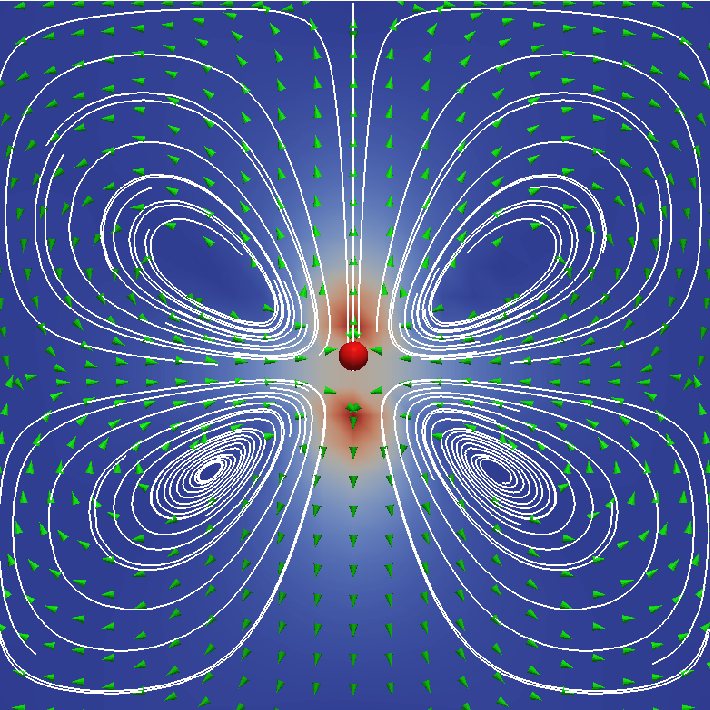
\includegraphics[width=0.5\columnwidth]{figures/flow_field.pdf}
\end{center}
\pagebreak
\definecolor{mygray}{gray}{.75}

 \tableofcontents
 \pagebreak
  
\section{Introduction}

%\floatingBox{5}{4cm}{Mein Text der in der Box abgebildet werden soll. Mal schauen wie das klappt.} 

Whether you are debugging a crashing simulation, trying to understand your simulation results, or create material to explain your findings to fellow researchers -- you are going to require ways to visualize what is going on in your system. Traditionally \ES{} has offered an interface to VMD (Visual Molecular Dynamics), a visualization package developed with NIH support by the Theoretical and Computational Biophysics group at the Beckman Institute, University of Illinois at Urbana-Champaign~\cite{vmd}.

While VMD is an incredibly powerful tool to visualize particle based data, it does not allow the user to include field data such as flow fields produced by coupled MD-LB simulations. To overcome this limitation, the lattice-Boltzmann and electrokinetics implementations in \ES{} contain output routines producing Paraview compatible VTK files. Routines to output particle positions exist as well, which allow the user to produce images and videos of coupled MD-continuum simulations.

\subsection*{Tutorial Outline}

At this stage, the tutorial only contains instructions on how to use Paraview with \ES{} generated data. Please to the User's Guide for information on how to visualize \ES{} simulations with VMD.

\pagebreak

\section{The LBM in brief}

\subsection*{Linearized Boltzmann equation}

Here we want to repeat a few very basic facts about the LBM. 
You will find much better introductions in various books and
articles, e.g. \cite{succi01a, duenweg09a}. It will however help clarifying 
our choice of words and we will eventually say something about the 
implementation in \ES{}. It is very loosely written, with the goal that
the reader understands basic concepts and how they are implemented in \ES{}.


The LBM essentially consists of solving a fully discretized
version of the linearized Boltzmann equation. The Boltzmann equation
describes the time evolution of the one particle distribution
function $f\left(x,p,t\right)$, which is the probability to find a molecule in a phase
space volume $\d x \d p$ at time $t$.The function $f$ is normalized
so that the integral over the whole phase space is the total 
mass of the particles:
\begin{equation*}
  \int f\left(x,p\right)\d x \d p = Nm,
\end{equation*}
where $N$ denotes the particle number and $m$ the particle mass.
The quantity f$\left(x,p\right)\d x \d p$ corresponds
to the mass of particles in this particular cell of the phase
space, the population. \\

\subsection*{Discretization}
The LBM discretizes the Boltzmann equation not only in real
space (the lattice!) and time, but also the velocity space is discretized.
A surprisingly small number of velocities, in 3D usually 
19, is sufficient to describe incompressible, viscous flow correctly.
Mostly we will refer to the three-dimensional model with a discrete
set of 19 velocities, which is conventionally called D3Q19.
These velocities, $\vec c_i$,
are chosen so that they correspond to the movement from one lattice
node to another in one time step. A two step scheme is used to transport
information through the system: In the streaming step
the particles (in terms of populations) are transported
to the cell where they corresponding velocity points to. 
In the collision step, the distribution functions
in each cell are relaxed towards the local thermodynamic
equilibrium. This will be described in more detail below.

\begin{figure}[htp]
\begin{center}
  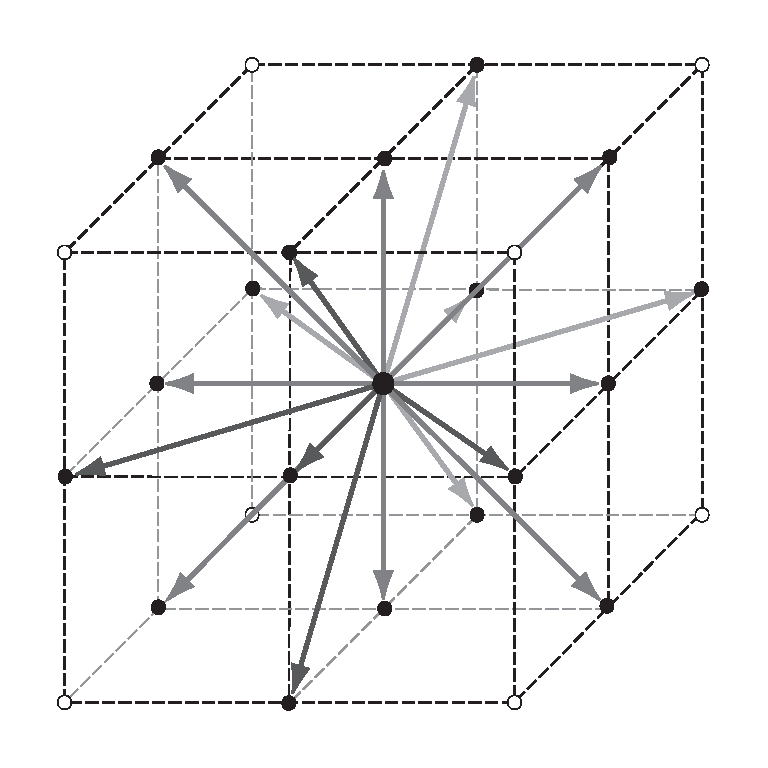
\includegraphics[height=0.3\textheight]{figures/latticeboltzmann-grid}
  \caption[]{The 19 velocity vectors $\vec{c}_{i}$ for a D$3$Q$19$ lattice. From
  the central grid point, the velocity vectors point towards all 18
  nearest neighbours marked by filled circles. The 19th velocity vector is the
  rest mode (zero velocity).}
  \label{fig:model-d3q18grid}
\end{center}
\end{figure}

The hydrodynamic fields, the density, 
the fluid momentum density,
the pressure tensor can be calculated straightforwardly from
the populations: They correspond to the moments
of the distribution function: 
\begin{align}
  \rho &= \sum f_i \\
  \vec{j} = \rho \vec{u} &= \sum f_i \vec{c_i} \\
  \Pi^{\alpha \beta} &= \sum f_i \vec{c_i}^{\alpha}\vec{c_i}^{\beta} 
  \label{eq:fields}
\end{align}
Here the Greek indices denotes the cartesian axis and the
Latin indices indicate the number in the disrete velocity set.
Note that the pressure tensor is symmetric.
It is easy to see that these equations are linear transformations
of the $f_i$ and that they carry the most important information. They
are 10 independent variables, but this is not enough to store the
full information of 19 populations. Therefore 9 additional quantities
are introduced. Together they form a different basis set of the
19-dimensional population space, the modes space and the modes are denoted by 
$m_i$. The 9 extra modes are referred to as kinetic modes or
ghost modes. It is possible to explicitly write down the 
base transformation matrix, and its inverse and in the \ES{}
LBM implementation this basis transformation is made for every
cell in every LBM step. It is possible to write a code that does not
need this basis transformation, but it has been shown, that this
only costs 20\% of the computational time and allows for 
larger flexibility.

\subsection*{The second step: collision}
The second step is the collision part, where
the actual physics happens. For the LBM it is assumed that
the collision process linearly relaxes the populations to the local
equilibrium, thus that it is a linear (=matrix) operator 
acting on the populations in each LB cell. It should conserve 
the particle number and the momentum. At this point it is clear
why the mode space is helpful. A 19 dimensional matrix that
conserves the first 4 modes (with the eigenvalue 1) is diagonal in the
first four rows and columns.
Some struggling with lattice symmetries shows that four independent
variables are anough to characterize the linear relaxation
process so that all symmetries of the lattice are obeyed. 
Two of them are closely related to 
the shear and bulk viscosity of the fluid, and two of them
do not have a direct physical equivalent. They are just called
relaxation rates of the kinetic modes.


The equilibrium distribution to which the populations relax 
is obtained from maximizing the information entropy 
$\sum f_i \log f_i$ under the constraint that the density
and velocity take their particular instantaneous 
values. 

In mode space the equilbrium distribution is calculated much from 
the local density and velocity.
The kinetic modes 11-19 have the value 0 in equilibrium.
The collision operator is diagonal in mode space
and has the form
\begin{align*}
  m^\star_i &= \gamma_i \left( m_i - m_i^\text{eq} \right) + m_i ^\text{eq}.
\end{align*}
Here $m^\star_i$ is the $i$th mode after the collision.
In words we would say: Each mode is relaxed towards
it's equilibrium value with a relaxation rate $\gamma_i$.
The conserved modes are not relaxed, or, the corresponding
relaxation parameter is one.

By symmetry consideration one finds that only four independent
relaxation rates are allowed. We summarize them here.
\begin{align*}
  m^\star_i &= \gamma_i m_i  \\
  \gamma_1=\dots=\gamma_4&=1 \\
  \gamma_5&=\gamma_\text{b} \\
  \gamma_6=\dots=\gamma_{10}&=\gamma_\text{s} \\
  \gamma_{11}=\dots=\gamma_{16}&=\gamma_\text{odd} \\
  \gamma_{17}=\dots = \gamma_{19}&=\gamma_\text{even} \\
\end{align*}

To include hydrodynamic fluctuations of the fluid, 
random fluctuations are added to the nonconserved modes $4\dots 19$ on every LB node so that
the LB fluid temperature is well defined and the corresponding
fluctuation formula, according to the fluctuation dissipation theorem holds.
An extensive discussion of this topic is found in \cite{duenweg07a}

\subsection*{Particle coupling}

Particles are coupled to the LB fluid with the force coupling:
The fluid velocity at the position of a particle is calculated 
by a multilinear interpolation and a force is applied on the particle
that is proportional to the velocity difference between particle 
and fluid:
\begin{equation}
  \vec{F}_D = - \gamma \left(v-u\right) 
  \label{eq:model-lbcoupling}
\end{equation}
The opposite force is distributed on the surrounding LB nodes. Additionally
a random force is added to maintain a constant temperature, according
to the fluctuation dissipation theorem. 
\begin{figure}[htp]
\begin{center}
   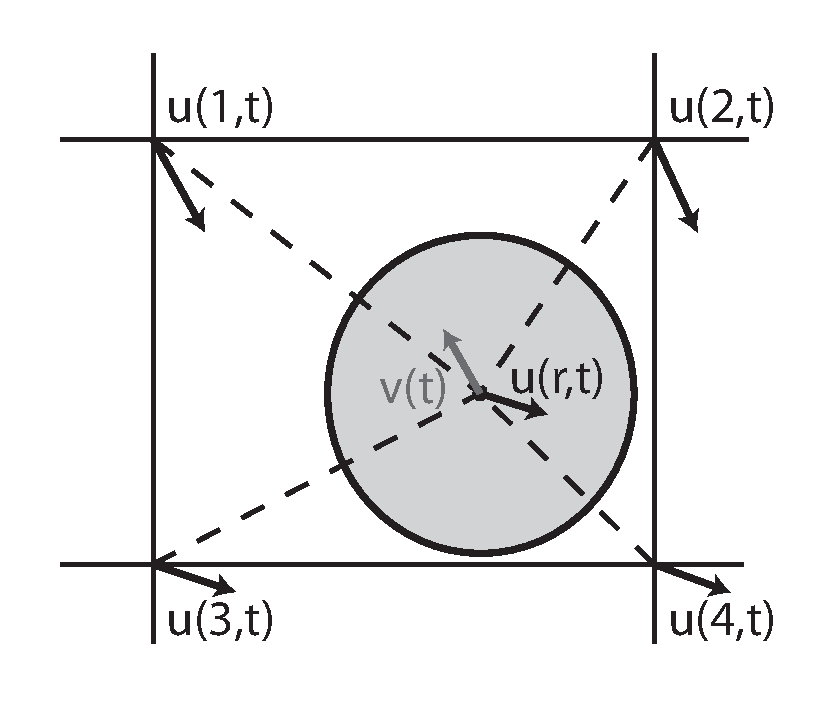
\includegraphics[height=0.3\textheight]{figures/latticeboltzmann-momentumexchange}
   \caption{The coupling scheme between fluid and particles is based on the
   interpolation of the fluid velocity $\vec{u}$ from the grid nodes.  
   This is done by linear interpolation. The difference between the
   actual particle velocity $\vec{v}(t)$ and the interpolated velocity
   $\vec{u}(\vec{r},t)$ is used in the momentum exchange of
   Equation~\ref{eq:model-lbcoupling}.}
  \label{fig:model-lbcoupling}
\end{center}
\end{figure}
\pagebreak



\section{The LB interface in \ES{}}
\ES{} features two virtually independent implementations of LB. One implementation
uses CPUs and one uses a GPU to perform the computational work. If in the first usage
of the command \texttt{lbfluid} the parameter \texttt{gpu} is given as first
parameter, the GPU will be used.

The LB lattice is a cubic lattice, with a lattice constant \texttt{agrid} that
is the same in all spacial directions. The chosen box length must be an integer multiple
of \texttt{agrid}. The LB lattice is shifted by 0.5 \texttt{agrid} in all directions: the node
with integer coordinates $\left(0,0,0\right)$ is located at
$\left(0.5a,0.5a,0.5a\right)$.
The LB scheme and the MD scheme are not synchronized: In one
LB time step typically several MD steps are performed. This allows to speed
up the simulations and is adjusted with the parameter \texttt{tau}.
The LB parameter \texttt{tau} must be an integer multiple of the MD timestep.

Even if MD features are not used a few MD parameters must be set, although they are irrelevant
to the LB module. These is mainly \texttt{skin}, but also the MD timestep has to be
set as the command \texttt{integrate} is used to propagate MD steps. LB steps are performed 
in regular intervals, such that the timestep $\tau$ for LB is recovered. 

\ES{} has three main commands for the LB module: 
 \texttt{lbfluid},  \texttt{lbnode}, and  \texttt{lbboundary}.
 \texttt{lbfluid} is mainly used to set up parameters and does everything that
concerns the whole fluid.  \texttt{lbnode} involves readout and manipulation of
single LB cells.  \texttt{lbboundary} allows to set boundaries, currently only
the bounce back boundary method is implemented to model
no-slip walls. Additionally the command  \texttt{thermostat lb} is used to set
the temperature. 


Important Notice: All commands of the LB interface use
MD units. This is convenient, as e.g. a particular 
viscosity can be set and the LB time step can be changed without
altering the viscosity. On the other hand this is a source
of a plethora of mistakes: The LBM is only reliable in a certain 
range of parameters (in LB units) and the unit conversion
may take some of them far out of this range. So note that you always
have to assure that you are not messing with that!

One brief example: a certain velocity may be 10 in MD units.
If the LB time step is 0.1 in MD units, and the lattice constant
is 1, then it corresponds to a velocity of 1 in LB units. 
This is the maximum velocity of the discrete velocity set and therefore
causes numerical instabilities like negative populations.

\subsection*{The \texttt{lbfluid} command}
The \texttt{lbfluid} command sets global parameters of the LBM. Every
parameter is given in the form \texttt{lbfluid name value}. 
All parameters except for \texttt{gamma\_odd} and  \texttt{gamma\_even}
are given in MD units. All parameters except for \texttt{ext\_force} accept
one scalar floating point argument. \\
\vspace{0,2cm}
\begin{tabular}{p{0.2\columnwidth}p{0.5\columnwidth}}
\texttt{dens} & The density of the fluid.\\
\texttt{grid} & The lattice constant of the fluid. It is used to determine the number of LB nodes 
per direction from \texttt{box\_l}. {\em They have to be compatible.} \\
\texttt{visc} & The kinematic viscosity \\
\texttt{tau} & The time step of LB. It has to be equal or larger than the MD time step. \\
\texttt{friction} & The friction coefficient $\gamma$ for the coupling scheme. \\
\texttt{ext\_force} & An external force applied to every node with three components. \\
\texttt{gamma\_odd} & Relaxation parameter for the odd kinetic modes. \\
\texttt{gamma\_even} & Relaxation parameter for the even kinetic modes.
\end{tabular} \\
\vspace{0,2cm}

A good starting point for an MD time step of 0.01 is the command line
\vspace{0,2cm}
\begin{lstlisting}[ numbers=none]
lbfluid grid 1.0 dens 10. visc .1 tau 0.01 friction 10.
\end{lstlisting}
\vspace{0,2cm}

\subsection*{The \texttt{lbnode} command}
The \texttt{lbnode} command allows to inspect and modify single LB nodes The
general syntax is:
\vspace{0,2cm}
\begin{lstlisting}[ numbers=none]
lbnode X Y Z command arguments
\end{lstlisting}
\vspace{0,2cm}
Note that the indexing in every direction starts with 0. The possible commands are:
\vspace{0,8cm}
\begin{tabular}{p{0.2\columnwidth}p{0.5\columnwidth}}
  print & Print one or several quantities to the TCL interface.\\
  set & Set one quantity to a particular value (can be a vector)\\
\end{tabular}\\
\vspace{0,8cm}
For both commands you have to specify what quantity should be printed
or modified. Print allows the following arguments: \\


\vspace{0,8cm}
\begin{tabular}{p{0.2\columnwidth}p{0.5\columnwidth}}
  \texttt{rho}\ & the density (scalar). \\
  \texttt{u} & the fluid velocity (three floats: $u_x$, $u_y$, $u_z$) \\
  \texttt{pi} & the fluid velocity (six floats: $\Pi_{xx}$, $\Pi_{xy}$, $\Pi_{yy}$, $\Pi_{xz}$,  $\Pi_{yz}$,  $\Pi_{zz}$) \\
  \texttt{pi\_neq} & the nonequilbrium part of the pressure tensor, components as above. \\
  \texttt{pop} & the 19 populations (check the order from the source code please).
\end{tabular} \\
\vspace{0,8cm}
Example:
The line
\vspace{0,2cm}
\begin{lstlisting}[ numbers=none]
puts [ lbnode 0 0 0 print u ]
\end{lstlisting}
\vspace{0,2cm}
prints the fluid velocity in node 0 0 0 to the screen.
The command \texttt{set} allows to change the density or fluid velocity in a single node. Setting
the other quantities can easily be implemented.
Example:
\begin{lstlisting}[ numbers=none]
puts [ lbnode 0 0 0 set u 0.01 0. 0.]
\end{lstlisting}
\subsection*{The \texttt{lbboundary} command}
The \texttt{lbboundary} command allows to set boundary conditions for the LB fluid. In general
periodic boundary conditions are applied in all directions and only if LB boundaries
are constructed finite geometries are used. This part of the LB implementation is still experimental,
so please tell us about your experience with it. In general even the simple case of no-slip
boundary is still an important research topic in the lb community and in combination with
point particle coupling not much experience exists. This means: Do research on that topic, play
around with parameters and find out what happens. 


The \texttt{lbboundary} command is supposed to resemble exactly the constraint command of 
\ES{}: Just replace the keyword \texttt{constraint} with the word \texttt{lbboundary} 
and \ES{} will create walls with the same shape as the corresponding constraint. Example:
The commands
\begin{lstlisting}[ numbers=none]
lbboundary wall dist 1.  normal 1. 0. 0. 
lbboundary wall dist -9.  normal -1. 0. 0. 
\end{lstlisting}
create a channel with walls parallel to the $yz$ plane with width 8.

Currently only the so called \emph{link bounce back} method is implemented, where the effective
hydrodynamic boundary is located midway between two nodes. This is the simplest and yet a 
rather effective approach for boundary implementation. The \texttt{lbboundary} command
checks for every LB node if it is inside the constraint or outside and flags it as a boundary
node or not. 

Currently only the shapes wall, sphere and cylinder are implemented but to implement others 
is straightforward. If you need them, please let us know.

\section{Drag force on objects}
As a first test, we measure the drag force on different objects in a simulation
box. Under low Reynolds number conditions, an object with velocity $\vec{v}$
experiences a drag force $\vec{F}_\text{D}$ proportional to the velocity:
\begin{align*}
	\vec{F}_\text{D}=-\gamma\vec{v},
\end{align*}
where $\gamma$ is denoted the friction coefficient. In general $\gamma$ is a
tensor thus the drag force is generally not parallel to the velocity. For
spherical particles the drag force is given by Stokes' law:
\begin{align*}
	\vec{F}_\text{D}=-6\pi\eta a\vec{v},
\end{align*}
where $a$ is the radius of the sphere.

In this task you will measure the drag force on falling objects with LB and
\ES{}. In the sample script \texttt{lb\_stokes\_force.tcl} a spherical object at rest
is centered in a square channel. Bounce back boundary conditions are assumed on
the sphere. At the channel boundary the velocity is fixed by using appropriate
boundary conditions. Within a few hundred or thousand  integration steps a
steady state develops and the force on the sphere converges.

\subsection*{Radius dependence of the drag force}
Measure the drag force for three different input radii of the sphere. How good
is the agreement with Stokes' law? Calculate an effective radius from Stokes'
law and the drag force measured in the simulation. Is there a clear relation to
the input radius? Remember how the bounce back boundary condition work and how
good spheres can be represented by them.

\subsection*{Visualization of the flow field}
The script produces \texttt{vtk} files of the flow field. Visualize the flow field
with \texttt{paraview}. Open \texttt{paraview} by typing it on the command line. Make
sure you are in the folder where the files are located. So the agenda is:
\begin{itemize}
	\item Click in the menu \texttt{File}, \texttt{Open...}
	\item Choose the files with flow field \texttt{fluid...vtk}
	\item Click \texttt{Apply}
	\item Add a stream tracer filter \texttt{Filters}, \texttt{Alphabetical},
	        \texttt{Stream tracer}
	\item Change the seed type from \texttt{point source} to \texttt{high resolution
		line source}
	\item Click \texttt{Apply}
	\item Rotate the visualization box to see the stream lines.
	\item Use the play button in the bar below the menu bar to show the time
		evolution.
\end{itemize}

\subsection*{System size dependence}
Measure the drag force for a fixed radius but varying system size. Does the drag
force increase of decrease with the system size? Can you find a qualitative
explanation?

\section{Polymer Diffusion}
In these exercises we want to use the LBM-MD-Hybrid to reproduce a classic
result of polymer physics: The dependence of the diffusion coefficient
of a polymer on its chain length. If no hydrodynamic interactions
are present, one expects a scaling law $D \propto N^{-1}$ and if 
they are present, a scaling law $D \propto N^{-\nu}$ is expected. 
Here $\nu$ is the Flory exponent that plays a very prominent role
in polymer physics. It has a value of $\sim 3/5$ in good solvent
conditions in 3D. Discussions of these scaling laws can be found
in polymer physics textbooks like \cite{degennes79a, doi96a, rubinstein03a}.


The reason for the different scaling law is the following:
When being transported, every monomer creates a flow field that follows
the direction of its motion. This flow field makes it easier 
for other monomers to follow its motion. This makes a polymer
long enough diffuse more like compact object including the fluid
inside it, although it does not have clear boundaries. It can be shown 
that its motion can be described by its hydrodynamic radius. It is defined 
as:
\begin{equation}
  \langle \frac{1}{R_h} \rangle = \langle \frac{1}{N^2}\sum_{i\neq j} \frac{1}{\left| r_i - r_j \right|} \rangle
\end{equation}
This hydrodynamic radius exhibits the scaling law  $R_h \propto N^{\nu}$
and the diffusion coefficient of long polymer is proportional to its inverse.
For shorter polymers there is a transition region. It can be described
by the Kirkwood-Zimm model:
\begin{equation}
  D=\frac{D_0}{N} + \frac{k_B T}{6 \pi \eta } \langle \frac{1}{R_h} \rangle
\end{equation}
Here $D_0$ is the monomer diffusion coefficient and $\eta$ the 
viscosity of the fluid. For a finite system size the second part of the
diffusion is subject of a $1/L$ finite size effect, because
hydrodynamic interactions are proportional to the inverse
distance and thus long ranged. It can be taken into account
by a correction:
\begin{equation}
  D=\frac{D_0}{N} + \frac{k_B T}{6 \pi \eta } \langle \frac{1}{R_h} \rangle \left( 1- \langle\frac{R_h}{L} \rangle \right)
  \label{kirkwood}
\end{equation}
It is quite difficult to prove this formula with good accuracy. It will 
need quite some computer time and a careful analysis. So please don't be
too disappointed if you don't manage to do so.


We want to determine the diffusion coefficient from the mean square
distance that a particle travels in the time $t$. For large $t$ it is
be proportional to the time and the diffusion coefficient occurs as 
prefactor: 
\begin{equation}
  \frac{\partial \langle r^2 \left(t\right)\rangle}{\partial t} = 2 d D. 
  \label{eq:msd}
\end{equation}
Here $d$ denotes the dimensionality of the system, in our case 3.
This equation can be found in virtually any simulation textbook, like
\cite{frenkel02b}.
We will therefore set up a polymer in an LB fluid, simulate for an appropriate
amount of time, calculate the mean square displacement as a function of
time and obtain the diffusion coefficient from a linear fit. However
we make a couple of steps in between and divide the full problem into 
subproblems that allow to (hopefully) fully understand the process.

\subsection{Step 1: Diffusion of a single particle}
Our first step is to investigate the diffusion of a single particle
that is coupled to an LB fluid by the point coupling method.
Take a look at the script \texttt{single\_particle\_diffusion.tcl}.
The script takes the LB-friction coefficient as an argument. Start with
an friction coefficient of 1.0:
{\vspace{0,2cm}\small
\begin{lstlisting}[numbers=none]
/path/to/Espresso single_particle_diffusion.tcl 1.0
\end{lstlisting}
\vspace{0,2cm}
}

In this script an LB fluid and a single particle are created and
thermalized. 
The random forces on the particle and
within the LB fluid will cause the particle to move. The mean squared
displacement is calculated during the simulation via a multiple-tau correlator. 
Run the simulation script and plot the output data \texttt{msd.dat} with
\texttt{gnuplot}.
What is different for short times than for long times?
Plot the data with double logarithmic axes.
{\vspace{0,2cm}\small
\begin{lstlisting}[numbers=none]
set log
plot "msd.dat"
\end{lstlisting}\vspace{0,2cm}
}
\begin{figure}[h]
  \begin{center}
	  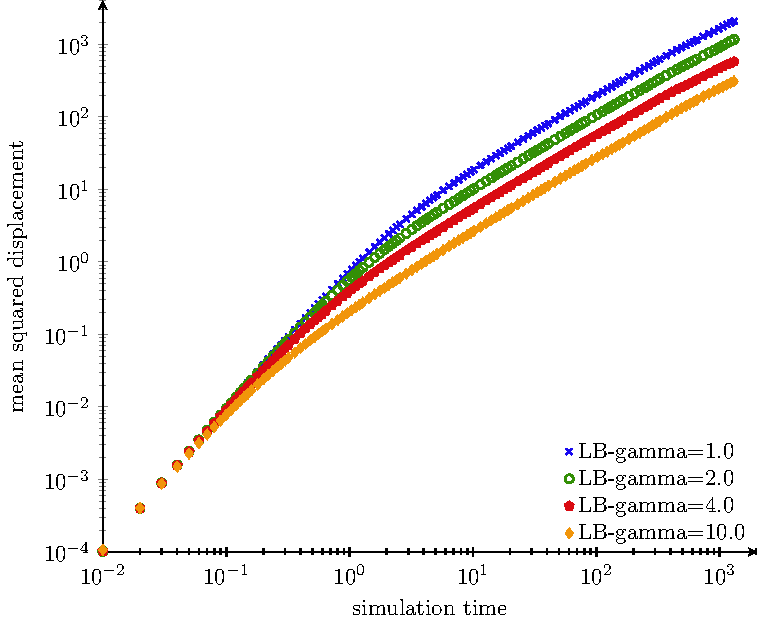
\includegraphics{figures/diffusion/msd.pdf}
  \end{center}
  \caption{Mean squared displacement of a single particle for different values
  of LB friction coefficient.}
\end{figure}

Can you give an explanation for the quadratic time dependency for short
times?
Use a linear fit in \texttt{gnuplot} for the long time regime to determine the 
diffusion coefficient:
{\vspace{0,2cm}\small
\begin{lstlisting}[numbers=none]
f(x)=a*x+b
fit [1:] f(x) 'msd.dat' via a,b
\end{lstlisting}\vspace{0,2cm}
}
The square brackets in the fit command tell \lstinline{gnuplot}
only to use the range right of $x=1$ for the fit. Choose the correct range by
yourself by looking at the log-log-plot of the MSD.

%The file \lstinline|energy.dat| contains the kinetic energy of the
%particle as a function of the elapsed simulation time. Investigate
%it, by plotting it with gnuplot. Calculate the average value of 
%the kinetic energy e.g. by fitting a constant function with gnuplot.
%What value would you expect from a working thermostat?

Run the simulation again with different values for the friction
coefficient, e.g. 1. 2. 4. 10. Calculate the diffusion
coefficient for all cases and use gnuplot to make a plot of
$D$ as a function of $\gamma$. What do you observe?
%The tiny helper script \lstinline|fit_lin.sh| 
%(with argument \lstinline|msd_pos.dat|)
%will help you with that. It contains
%a (quite ugly) gnuplot one-liner that does the fitting and just
%returns the slope. The fit is performed in the range 5 to 40 that
%has proved to work good for runs of $\sim 100000$ steps. You have to 
%modify the script to change that range.
%Is there any difference between the
%friction coefficient that you put in, and the diffusion coefficient
%you obtain?

%\section{Step 3: The long time tail of the velocity autocorrelation function}
%Should we do anything here?

\subsection{Step 2: Diffusion of a polymer}
One of the typical applications of \ES{} is the simulation of polymer chains 
with a bead-spring-model. For this we need a repulsive interaction
between all beads, for which one usually takes a shifted and truncated
Lennard-Jones (so called Weeks-Chandler-Anderson) interaction, 
and additionally a bonded interaction between 
adjacent beads to hold the polymer together. You have already learned
that the command
{\vspace{0,2cm}\small
\begin{lstlisting}[numbers=none]
inter 0 0 lennard-jones 1. 1. 1.125 0.25 0. 
\end{lstlisting}\vspace{0,2cm}
}
creates a Lennard-Jones interaction with $\varepsilon=1.$, $\sigma=1.$,
$r_\text{cut} = 1.125$ and $\varepsilon_\text{shift}=0.25$ between particles
of type 0, which is the desired 
repulsive interaction. The command
{\vspace{0,2cm}\small
\begin{lstlisting}[numbers=none]
inter 0 FENE 7. 2. 
\end{lstlisting}\vspace{0,2cm}
}
creates a FENE (see \ES{} manual for the details) bond interaction. Still \ES{}
does not know between which beads this interaction should be applied.
This can be either be specified explicitly or done with the \lstinline|polymer|
command. This creates a given number of beads, links them with the given
bonded interaction and places them following a certain algorithm. We will
use the pruned self-avoiding walk: The monomers are set according 
to a pruned self-avoiding walk (in 3D) with a
fixed distance between adjacent bead positions. The syntax is:
{\vspace{0,2cm}\small
\begin{lstlisting}[numbers=none]
polymer $N_polymers $N_monomers 1.0 types 0 mode PSAW bond 0 
\end{lstlisting}\vspace{0,2cm}
}
Using a random walk to create a polymer causes trouble: The random walk may 
cross itself (or closely approach itself) and the LJ potential is very
steep. This would raise the potential energy enormously and would make
the monomers shoot through the simulation box. The pruned self-avoiding
walk should prevent that, but to be sure
we perform some MD steps with a capped LJ potential, this means 
forces above a certain threshold will be set to the threshold in order to prevent
the system from exploding. To see how this is done, look at the script 
\texttt{polymer\_diffusion.tcl}.
It contains a quite long warmup command so that also longer polymers
are possible. You can probably make it shorter.

It is called in the following way:
{\vspace{0,2cm}\small
\begin{lstlisting}[numbers=none]
/path/to/Espresso polymer_diffusion.tcl $N_monomers  
\end{lstlisting}\vspace{0,2cm}
}
This allows to quickly change the number of monomers without editing 
the script. Change the variable  \lstinline|vmd_output| to yes to 
look at the diffusing polymer.
For the warmup a Langevin thermostat is used to keep the temperature constant.
You will have to add the LB command by yourself.
Furthermore we want to compute the diffusion constant of the polymer for
different numbers of monomers. For this purpose we can again use the multiple
tau correlator. Have a look at the \ES{} -script for the single particle diffusion
and add the adapted commands for the polymer. Find out how many integration steps are
necessary to capture the long-time diffusion regime of the polymer. The script
already computes the time averaged hydrodynamic radius and stores it in a file
\lstinline|rh_nomX.dat| where \lstinline|X| is the number of monomers.

Run the script for different numbers of monomers and use gnuplot to calculate
the diffusion coefficient as a function of the chain length. Compare the results
of your \ES{} simulations with the given Kirkwood-Zimm formula
(eq.~\ref{kirkwood}).

\documentclass[11pt, tikz]{standalone}
\usepackage[english]{babel}
\usepackage[utf8]{luainputenc}
\usepackage{graphicx}
%\usepackage{subcaption}
\usepackage{amssymb}
\usepackage{amsmath}
\usepackage{hyperref}
\usepackage{breakurl}
\usepackage{amstext}
\usepackage{color}
\usepackage{transparent}
%\usepackage{float}
\usepackage{caption}
%\usepackage{textcomp}
%\usepackage[sorting=none,backend=biber]{biblatex}
%\usepackage{csquotes}
\usepackage{siunitx}
%\usepackage{framed}
%\usepackage{listings}
%\usepackage{ifthen}
%\usepackage{xkeyval}
%\usepackage{calc}
%\usepackage{todonotes}
%\usepackage{letltxmacro}
%
%\bibliographystyle{plain}
%%%%%% plotting %%%%%%%%%%%%%%%%%%
\usepackage{pgfplots}
\usepackage{pgfplotstable}
\usepackage{tikz}
\usetikzlibrary{backgrounds, arrows, positioning, intersections, fit, pgfplots.groupplots, spy, matrix, calc}
\pgfplotsset{compat=newest}
%\usepgfplotslibrary{external}
%\tikzset{external/system call={lualatex
%\tikzexternalcheckshellescape -halt-on-error -interaction=batchmode
%-jobname "\image" "\texsource"}}
%\tikzexternalize[prefix=./images/]
%
%%%%%%%%% Solving problem of externalize and package 'todonotes'
%\LetLtxMacro{\oldmissingfigure}{\missingfigure}
%\renewcommand{\missingfigure}[2][]{\tikzexternaldisable\oldmissingfigure[{x}]{#2}\tikzexternalenable}
%
%\LetLtxMacro{\oldtodo}{\todo}
%\renewcommand{\todo}[2][size=\small]{\tikzexternaldisable\oldtodo[x]{#2}\tikzexternalenable}
\newcommand{\kb}{k_\textnormal{B}}
%%%%%%%%%%%%%%%%%%%%%%%%%%%%%%%%%%%%%%%%%%%%%%%%%%%%%%%%%%%%%%%%%%%%%%%%%%%%%%%%%%%%%%%%%%%%%%%%%%
\setlength{\marginparwidth}{3cm}
%define paper colors
\definecolor{paper_01}{HTML}{1809F0}
\definecolor{paper_02}{HTML}{338F06}
\definecolor{paper_03}{HTML}{DA0B12}
\definecolor{paper_04}{HTML}{F1950A}
\definecolor{paper_05}{HTML}{A9D81D}
\definecolor{paper_06}{HTML}{F56B20}

%define bright color palette
\definecolor{custom_0_00}{HTML}{8585DD}
\definecolor{custom_0_01}{HTML}{99CC01}
\definecolor{custom_0_02}{HTML}{E20C53}
\definecolor{custom_0_03}{HTML}{66056B}
\definecolor{custom_0_04}{HTML}{044749}
\definecolor{custom_0_05}{HTML}{DBB30B}
\definecolor{custom_0_06}{HTML}{6B320B}
\definecolor{custom_0_07}{HTML}{919B08}
\definecolor{custom_0_08}{HTML}{589FAF}
\definecolor{custom_0_09}{HTML}{C17A3A}
%define medium color palette
\definecolor{custom_1_00}{HTML}{B4B3E0}
\definecolor{custom_1_01}{HTML}{C5E507}
\definecolor{custom_1_02}{HTML}{E46288}
\definecolor{custom_1_03}{HTML}{83518C}
\definecolor{custom_1_04}{HTML}{1F6666}
\definecolor{custom_1_05}{HTML}{DCC252}
\definecolor{custom_1_06}{HTML}{6C5646}
\definecolor{custom_1_07}{HTML}{989E6D}
\definecolor{custom_1_08}{HTML}{91ACB5}
\definecolor{custom_1_09}{HTML}{C49E76}
%define pale color palette
\definecolor{custom_2_00}{HTML}{E9E9F2}
\definecolor{custom_2_01}{HTML}{E7FF80}
\definecolor{custom_2_02}{HTML}{FFC2D9}
\definecolor{custom_2_03}{HTML}{C692CC}
\definecolor{custom_2_04}{HTML}{64B0B2}
\definecolor{custom_2_05}{HTML}{F2E5AF}
\definecolor{custom_2_06}{HTML}{B2A29A}
\definecolor{custom_2_07}{HTML}{BEBFA5}
\definecolor{custom_2_08}{HTML}{C0DEE2}
\definecolor{custom_2_09}{HTML}{E5D5C3}
%define SimTech colors
\definecolor{simtech_blue}{HTML}{879DC4}
\definecolor{simtech_orange}{HTML}{F15D27}
%define colors for code listings
\definecolor{mygreen}{rgb}{0,0.4,0}
\definecolor{mygray}{rgb}{0.5,0.5,0.5}
\definecolor{lightgray}{rgb}{0.9,0.9,0.9}
\definecolor{mymauve}{rgb}{0.58,0,0.82}
\definecolor{myred}{HTML}{B02A2C}
\definecolor{mypink}{HTML}{FF53FF}
\definecolor{myblue}{HTML}{0B0BC8}
%
\definecolor{warningred}{HTML}{FF0000}
% colwidth is 221 for 11pt article, we use 1.5*colwidth
\newlength{\plotwidth}
\setlength{\plotwidth}{330pt}
\pgfplotsset{every x tick/.append style={color=black, thick}}
\pgfplotsset{axis line style={thick}}
%\pgfplotsset{width=\plotwidth}
\pgfplotsset{width=\textwidth}
%
\tikzset{every pin/.style={fill=lightgray,rectangle,rounded
	corners=3pt}}
\pgfplotsset{%
	every axis/.append style={mark=x, line width=.8pt, scaled ticks=false, tick label style={/pgf/number format/fixed}},
	every axis legend/.append style={nodes={right},draw=none, fill=none},
	every mark/.append style={solid},
	mystyle1/.style ={solid, mark=x, mark options={solid, scale=1.0}, line width=.8pt},
	%mystyle2/.style ={dotted, mark=x, mark options={solid}},	
	mystyle2/.style ={solid, mark=o, mark options={solid, scale=1.0}, line width=.8pt},	
	%mystyle3/.style ={dashed, mark=x, mark options={solid}},
	mystyle3/.style ={solid, mark=pentagon*, mark options={solid, scale=1.0}, line width=.8pt},
	%mystyle4/.style ={dashdotted, mark=x, mark options={solid}},
	mystyle4/.style ={solid, mark=diamond*, mark options={solid, scale=1.0}, line width=.8pt},
	%mystyle5/.style ={dashdotdotted, mark=x, mark options={solid}},
	mystyle5/.style ={solid, mark=square*, mark options={solid, scale=1.0}, line width=.8pt},
}



\begin{document}
\begin{tikzpicture}
	\pgfplotsset{
		legend style = {
		at={(1.0,1.0)},
		anchor=north east
		}}
	\begin{axis}
		[minor tick num=1,
		axis x line=bottom,
		axis y line = left,
		xlabel = {x position},
		xmin = 0.0,
		xmax = 16.0,
		ylabel = {LB fluid velocity}, 
		ymin = 0.0,
		ymax = 0.02,
		]
		\addplot+[color=paper_01, mystyle1, only marks] file {./fluid_velocity.dat};
		\addplot+[color=paper_02, samples=500, no marks, domain=1.5:13.5] 
		{0.001/2.0*(12^2/4.0-(x-7.5)^2)};
		\legend{data,analytical prediction};
	\end{axis}
\end{tikzpicture}
\end{document}

\clearpage
\bibliographystyle{unsrt}
\bibliography{refs}
\end{document}

